\documentclass{article}
\usepackage{graphicx}
\usepackage{siunitx}
\graphicspath{ {images/} }
\title{Ball Rolling}
\author{Grant Curell}
\begin{document}
\maketitle{}
\section{Problem}
Suppose you know that a ball is rolling on a flat table at \ang{15} from a direction parallel to the bottom edge with a speed of 7.0 meters/second. You may want to find out how long the ball will take to roll off the edge 1.0 meter to the right.
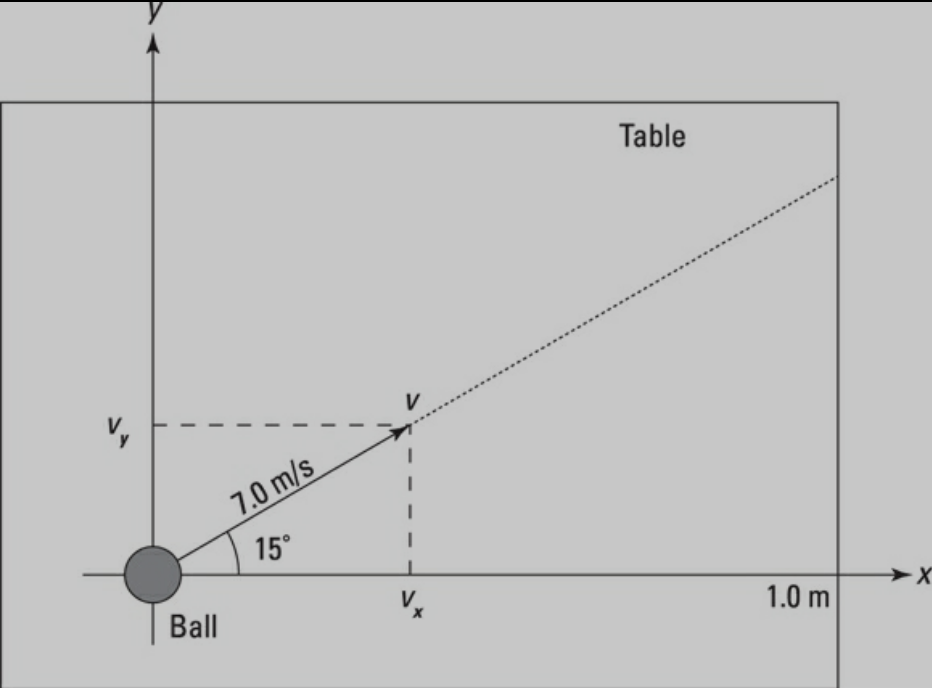
\includegraphics[width=\columnwidth]{image}
\\\\
Holzner, Steven. Physics I For Dummies (For Dummies (Math \& Science)) (p. 58). Wiley. Kindle Edition.
\\\\
\section{Solution}
\[ \cos(15) = \frac{x}{7m/s} \]
\[ x=6.76 \]
\[ s=\bar{v}t \]
\[ \frac{1}{6.76}=t \]

\end{document}
